\begin{ledgroupsized}[r]{120mm}
\footnotesize 
                \pstart                
                \noindent\textbf{\"{U}berlieferung:}   
                \pend
                \end{ledgroupsized}
            
              
                           \begin{ledgroupsized}[r]{114mm}
                            \footnotesize 
                            \pstart \parindent -6mm
                            \makebox[6mm][l]{\textit{L}}Konzept: LH XXXVIII Bl. 170-171.
1 Bog. 4\textsuperscript{o}, beschnitten.
2~S. auf Bl.~170.
Bl.~171~r\textsuperscript{o} überliefert N.~90. %?? = LH038_171r (De horologiis communibus)
Bl.~171~v\textsuperscript{o} ist leer.
\\Cc 2, Nr. 00 \pend
                                                        \end{ledgroupsized}
                                                         
                %\normalsize
                \vspace*{5mm}
                \begin{ledgroup}
                \footnotesize 
                \pstart
            \noindent\footnotesize{\textbf{Datierungsgr\"{u}nde}: Das vorliegende Stück N.~91 %?? = LH038_170 (De horologiis pendulis)
nimmt auf Christiaan Huygens' \cite{00123}\title{Horologium oscillatorium} bezug.
Ein druckfrisches Exemplar dieser Abhandlung bekam Leibniz wahrscheinlich Anfang April 1673 geschenkt,
als er Huygens in Paris besuchte.
Seine Randbemerkungen darin sowie mannigfaltige Hinweise in mathematischen Aufzeichnungen zeigen,
dass er sich noch in den Monaten April und Mai 1673 mit dem \cite{00123}\title{Horologium oscillatorium} auseinandergesetzt hat.
(Siehe hierüber \cite{00262}\textit{LSB} VII,~4 N.~2, S.~27.)
Auch N.~91 %?? = LH038_170 (De horologiis pendulis)
d\"{u}rfte in diesem Zeitraum entstanden sein,
wie dies insbesondere aus dem Incipit hervorgeht.
}
                \pend
                \end{ledgroup}
            
                \vspace*{8mm}
                \pstart%
\normalsize%
% \begin{center}%
\noindent%
[170~r\textsuperscript{o}]
\pend%
\pstart%
\noindent%
\centering%
De Horologiis pendulis, non tam aequalibus quam creduntur
% \end{center}%
\pend%
\vspace{0,5em}%
\pstart%
\noindent%
Cum nuper Horologia pendula diligentius considerassem et a cl.
\edtext{Hugenio\protect\index{Namensregister}{\textso{Huygens} (Hugenius, Ugenius, Hugens, Huguens), Christiaan 1629-1695}%
}{\lemma{Hugenio}\Cfootnote{\cite{00123}\textsc{C. Huygens}, \textit{Horologium oscillatorium}, Amsterdam 1673, S.~6 (\textit{HO} XVIII, S.~95).}}
\edtext{fol. 6.}{\lemma{fol. 6.}\Bfootnote{\textit{erg. L}}}
asseri animadvertissem, tantam esse eorum aequalitatem,
ut \textit{vel recte tempus metiantur, vel omnino non metiantur};
ita, ut jactatio navis proinde non noceat, modo
\edtext{motus non interruptus}{\lemma{motus}\Bfootnote{\textbar\ non \textit{erg.} \textbar\ interruptus \textit{L}}}
servetur; hoc quia mihi permirum videbatur, quaesivi an alicubi demonstrasset.
Cumque nuspiam ab eo id probari viderem, magnus enim pulcherrimarum
\edtext{sane}{\lemma{sane}\Bfootnote{\textit{erg. L}}}
demonstrationum apparatus tantum oscillationum spontanearum a sola descendentis gravitate ortarum
\edtext{isochronismum ostendit;}{\lemma{isochronismum}\Bfootnote{\textit{(1)}\ probat \textit{(2)}\ ostendit; \textit{L}}}
in rem hanc
\edtext{inquisivi curatius,}{\lemma{inquisivi}\Bfootnote{\textit{(1)}\ diligentius \textit{(2)}\ curatius, \textit{L}}}
tandemque aliud
\edtext{plane}{\lemma{plane}\Bfootnote{\textit{erg. L}}}
dicendum deprehendi.
\pend
                         \pstart 
                                    Ponamus Pendulum ex aliquo puncto ut \textit{A} libere solo suo pondere demissum oscillationes aliquot
\edtext{peragere, ut $AD,$ $BE,$ easque concedamus (ob cycloides eas) esse isochronas,}%
{\lemma{peragere,}\Bfootnote{%
\textit{(1)}\ eas %
\textit{(2)}\ ut \textit{AD}, \textit{BE}, easque %
\textit{(a)}\ esse isochronas %
\textit{(b)}\ concedamus (ob cycloides \textbar\ eas \textit{erg.} \textbar\ ) esse isochronas, \textit{L}}}
nulla resistentiae aeris erga penetrationem, aut fili contra flexionem,
aut axis contra gyrationem in polis, habita ratione, modo vi solius gravitatis moveatur.
  \pend
  \newpage
  \pstart
  \noindent
 \begin{wrapfigure}[8]{lH}{0.35\textwidth} 
 \vspace{-4mm}
 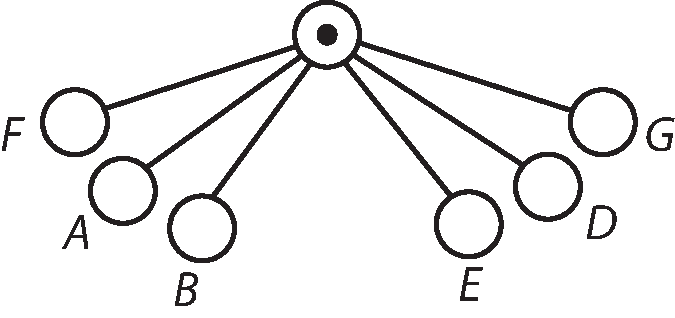
\includegraphics [trim = -3mm 3mm -13mm 0mm, clip, width=0.38\textwidth] {images/lh038_170v.pdf}
\begin{center} [\textit{Fig. 1}]\\
 \end{center}
%\caption{Bildbeschreibung}
\end{wrapfigure}
Nunc vero ponamus pendulum ex puncto \textit{A} initio libere demissum vi solius quidem gravitatis
\edtext{moveri coepisse,}{\lemma{moveri}\Bfootnote{\textbar\ facile \textit{gestr.} \textbar\ coepisse, \textit{L}}}
sed durantibus oscillationibus cum ex \textit{B} nisu
\edtext{gravitatis descendere inciperet,}%
{\lemma{gravitatis}\Bfootnote{%
\textit{(1)}\ descendens pervenisset in \textit{C} %
\textit{(2)}\ descendere inciperet, \textit{L}}}
ibi accipere ictum a rota horologii,
ac proinde majori celeritate descensum continuare quam alias fecisset
eoque motu non excurrere tantum usque ad \textit{E}, sed altius adhuc usque ad \textit{G}.
\pend 
\count\Bfootins=1050
\pstart  Porro si impetus a rota impressus non sit nimius (quod utique caveri potest ac debet) tunc utique
\edtext{assumi poterit}{\lemma{assumi poterit}\Bfootnote{\textit{erg. L}}}
alia oscillatio \textit{FG} talis, ut pendulum ex puncto \textit{F} (recte ad hoc assumto) demissum,
libere nisu gravitatis eandem collegisset celeritatem, ubi venisset in \textit{B}, quam nunc ibi
\edtext{acquisivit %
[170~v\textsuperscript{o}]
impetu rotae impresso.}{\lemma{acquisivit}\Bfootnote{%
\textit{(1)}\ partim [170~v\textsuperscript{o}] descensu a $B$ ad $C$, partim %
\textit{(2)}\ impetu rotae impresso. \textit{L}}}
Et proinde vi hujus oscillationis pendulum etiam necessario pervenisset usque
\edtext{ad \textit{G}, eadem enim vis}{\lemma{ad \textit{G},}\Bfootnote{%
\textit{(1)}\ cum eadem %
\textit{(2)}\ eadem enim \textit{L}}}
quam pendulum habet
\edtext{in \textit{B} eodemque tendens undecunque orta ipsum eodem}%
{\lemma{in \textit{B}}\Bfootnote{%
\textit{(1)}\ undecunque orta %
\textit{(a)}\ ipsum eodem %
\textit{(b)}\ eodemque tendens, %
\textit{(2)}\ eodemque [...] eodem \textit{L}}}
elevabit, nempe in \textit{G}.
Haec oscillatio \textit{FG} utique erit aequidiuturna oscillationi spontaneae \textit{BE} vel \textit{AD}.
Sed \edtext{eadem \textit{FG} diuturnior}{\lemma{eadem}\Bfootnote{%
\textit{(1)}\ longior %
\textit{(2)}\ \textit{FG} diuturnior \textit{L}}}
esset parte sui \textit{BG},
quae cum sit aequidiuturna oscillationi praesenti \textit{BG} quae ab impetu rotae
\edtext{gravitati accedente}{\lemma{gravitati accedente}\Bfootnote{\textit{erg. L}}}
orta est, sequitur oscillationem \textit{FG},
adeoque et oscillationem \textit{AD} vel \textit{BE} diuturniorem esse oscillatione
\edtext{\textit{BG}}{\lemma{\textit{BG}}\Bfootnote{\textit{erg. L}}}
orta ab impetu rotae gravitati accedente,
ac proinde oscillationes ab inaequalibus impressionibus rotarum horologii,
aut jactationum navis, aliisque hujusmodi causis reddi inaequales.
Quod demonstrandum sumseramus.
Itaque quo
\edtext{major in pendulis obtineatur aequalitas,}{\lemma{major}\Bfootnote{%
\textit{(1)}\ pendulis %
\textit{(a)}\ detur %
\textit{(b)}\ inaequalitatis %
\textit{(2)}\ in pendulis obtineatur aequalitas, \textit{L}}}
adhibendum erit praeterea artificium meum,
\edtext{quo efficitur,}{\lemma{quo}\Bfootnote{%
\textit{(1)}\ alternis %
\textit{(2)}\ efficitur, \textit{L}}}
ut impetus pendulo vel elastro, eorumve libramento impressus sit semper idem.
Machina Horologii pondus aliquod vel Elastrum exiguum, tantisper
\edtext{dum libramentum}{\lemma{dum}\Bfootnote{%
\textit{(1)}\ pendulum %
\textit{(2)}\ libramentum \textit{L}}}
vibratur restituente, ut
\edtext{postea ad rediens libramentum, novo ictu priorem aequante percutiendum sit paratum.}%
{\lemma{postea}\Bfootnote{%
\textit{(1)}\ rediens libramentum paratum %
\textit{(2)}\ ad rediens [...] paratum. \textit{L}}}
Ex his ratio redditur ejus quod ipse fatetur Hugenius,\protect\index{Namensregister}{\textso{Huygens}, Christiaan (1629-1695)}
quo minore vi pendula motum continuare possunt, eo esse exactiora;
quod non esset, si vis impressa non turbaret.\pend
\count\Bfootins=1500
 


 


 


 

